%\bigskip
%\hrule
%\smallskip
%\hfill Edited by Takayoshi Shoudai on 2024-05-18 (2nd version), 2024-10-30 (3rd version)
\subsection{Characteristic sets for finite union of regular patterns}\label{subsec:char_union}

\begin{figure*}[t]
  \begin{center}
    %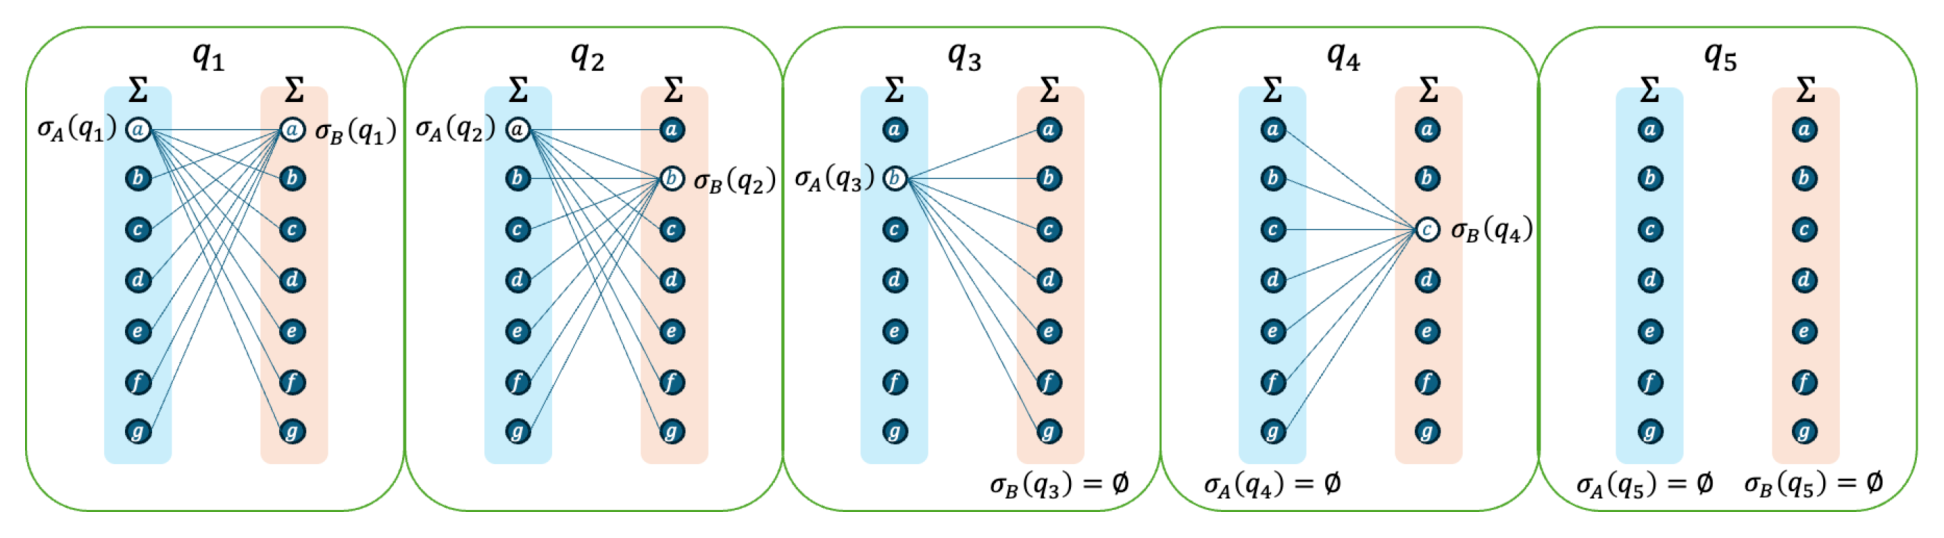
\includegraphics[scale=0.5]{figs/lem8eachreg.eps}
    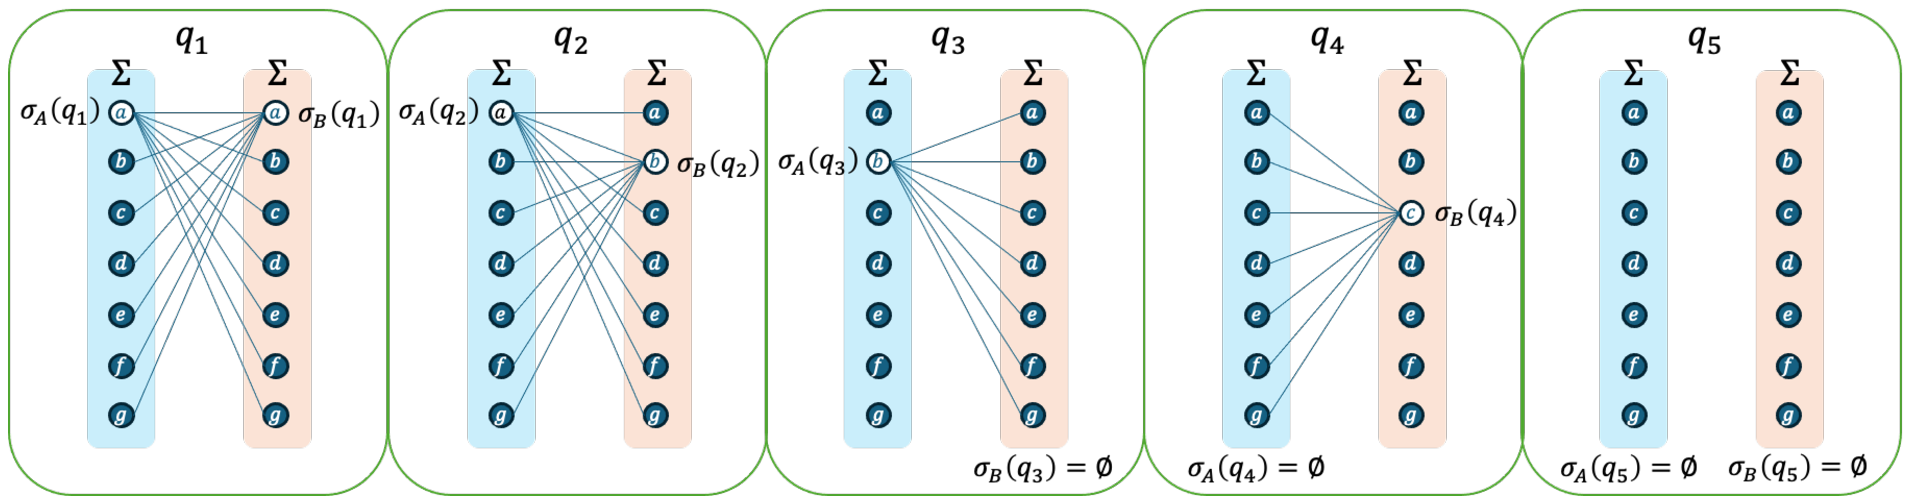
\includegraphics[scale=0.54]{figs/lem8eachreg.pdf}
    \caption{Let $\Sigma=\{a,b,c,d,e,f,g\}, Q=\{q_1,q_2,q_3,q_4,q_5\}$. We set $A(q_1)=\{a\}$ and $B(q_1)=\{a\}$, and then $\sigma_A(q_1)=a$ and $\sigma_B(q_1)=a$, and so on. For each regular pattern $q_i$ ($i=1,\ldots,5$), we represent a string $w \in \Sigma\cdot\Sigma$ satisfying that $p\{x:=w\}\preceq q_i$ by the edge between the left (first) and right (second) symbols of $w$. For example, the leftmost figure shows that $p\{x:=ay\}\preceq q_1$ and $p\{x:=ya\}\preceq q_1$ for a variable symbol $y$. We note that these figures may contain more edges than those illustrated. From these figures, we get $\ell_A=1, \ell_B=0$, and $Q^{(\bot,\bot)}=\{q_5\}, Q^{(\bot,\cdot)}=\{q_4\}, Q^{(\cdot,\bot)}=\{q_3\}, Q^{(\cdot,\cdot)}=\{q_1,q_2\}$.}\label{fig:lem8eachreg}
  \end{center}
\end{figure*}

\begin{figure}[t]
  \begin{center}
    %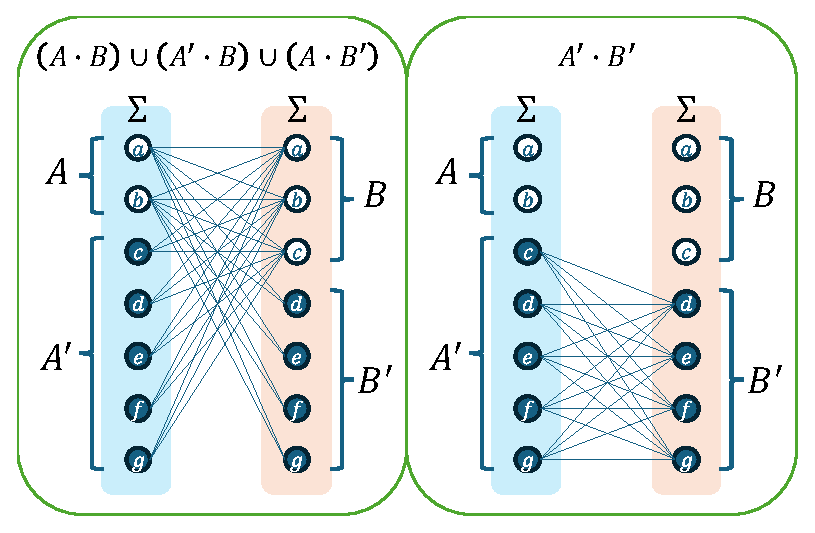
\includegraphics[scale=0.5]{figs/lem8totalreg.eps}
    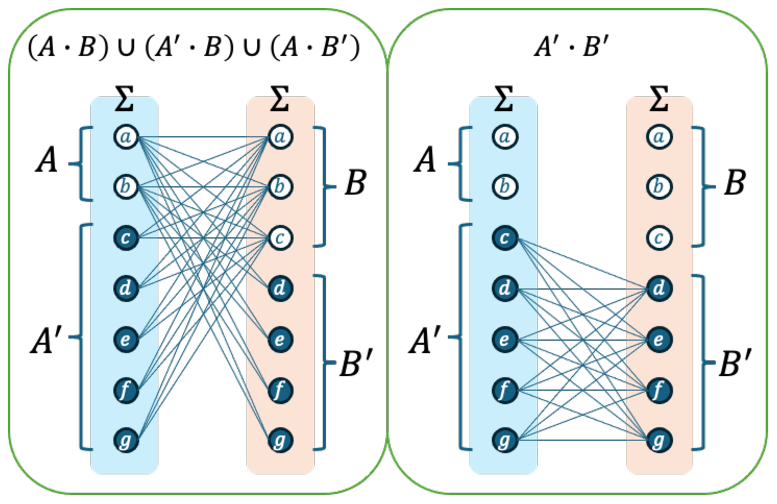
\includegraphics[scale=0.525]{figs/lem8totalreg.pdf}
    \caption{In the left figure, we aggregate all of the edges appearing in Fig.~\ref{fig:lem8eachreg}. For all $w=a'b'\in A'\cdot B'$, there must be a regular pattern $q_i$ $(1\leq i\leq 5$) that satisfies that $p \{ x:=w \} \preceq q_i$.}\label{fig:lem8totalreg}
  \end{center}
\end{figure}

\begin{lem}\label{追加補題1}
Let $k$ be an integer with $k\geq 1$.
Let $\Sigma$ be an alphabet with $\sharp \Sigma = k + 2$.
Let $p \in \RPat$ in which a variable symbol $x$ appears, and let $Q \in \RPat^{k}$.
If for any string $w \in \Sigma^{\ast}$ with $|w|=2$, there exists a regular pattern $q_{w} \in Q$ such that $p \{ x:=w \} \preceq q_{w}$ holds, then there exists a regular pattern $q \in Q$ such that $p \{ x:=xy \} \preceq q$ holds, where $y$ is a variable symbol that does not appear in $q$.
\end{lem}

\begin{proof}
Without loss of generality, we suppose that $\sharp Q = k$ holds. Otherwise, for some regular pattern $q$ already in $Q$, we can add a new regular pattern $q'$ equivalent to $q$, i.e., $q' \equiv q$, to $Q$ repeatedly until $\sharp Q = k$ is satisfied.
For any $q \in Q$, we define the sets $A(q), B(q) \subseteq \Sigma$ as follows:
\begin{align*}
  A(q) & = \{ a \in \Sigma \mid p \{ x:=ay \} \preceq q,\ y\in X\},\\ 
  B(q) & = \{ b \in \Sigma \mid p \{ x:=yb \} \preceq q,\ y\in X\}.
  \end{align*}
If there exists $q\in Q$ such that $|A(q)|\geq 2$ or $|B(q)|\geq 2$, from Lemma~\ref{lem:twovariables}, $p\{x := xy\} \preceq q$ holds.
Below, we suppose that $|A(q)|\leq 1$ and $|B(q)|\leq 1$.
Let $\bot$ be a constant symbol that is not a member in $\Sigma$.
We define the functions $\sigma_{A}: Q \rightarrow \Sigma \cup \{\bot\}$ and $\sigma_{B}: Q \rightarrow \Sigma \cup \{\bot\}$ as follows:
\begin{align*}
  \sigma_{A}(q) & =
  \begin{cases}
    a & \textrm{if } A(q) = \{a\}, \\
    \bot & \textrm{if } A(q) = \emptyset.
  \end{cases}\\
  \sigma_{B}(q) & =
  \begin{cases}
    b & \textrm{if } B(q) = \{b\}, \\
    \bot & \textrm{if } B(q) = \emptyset.
  \end{cases}
\end{align*}
The inverse functions of $\sigma_{A}$ and $\sigma_{B}$ are denoted by $\sigma_{A}^{-1}$ and $\sigma_{B}^{-1}$, respectively. That is, for $a,b \in \Sigma \cup \{\bot\}$, let $\sigma_{A}^{-1}(a) = \{q \in Q \mid \sigma_{A}(q) = a\}$ and $\sigma_{B}^{-1}(b) = \{q \in Q \mid \sigma_{B}(q) = b\}$. 
We give an example in Fig.~\ref{fig:lem8eachreg}.

$A$ and $B$ denotes the following subsets of $\Sigma$:
\begin{align*}
  A & = \bigcup_{q \in Q \setminus \sigma_{A}^{-1}(\bot)} A(q) \mbox{,~~~}
  B = \bigcup_{q \in Q \setminus \sigma_{B}^{-1}(\bot)} B(q).
\end{align*}
Then, let $A' = \Sigma \setminus A$ and $B' = \Sigma \setminus B$.
For any $a,b \in \Sigma$, we use the following notations:
\begin{align*}
  %\ell_{A}(a) & = \{ q \in Q \mid p \{ x:=ay \} \preceq q,\ y\in X\},\\ 
  %\ell_{B}(b) & = \{ q \in Q \mid p \{ x:=yb \} \preceq q,\ y\in X\}\\
  %\ell_{A} &= \sum_{a \in \Sigma}(\ell_{A}(a) - 1),\\
  \ell_{A} &= \sum_{a \in A}(\sharp \sigma_{A}^{-1}(a) - 1) \mbox{,~~~}
  %\ell_{B} &= \sum_{b\in \Sigma}(\ell_{B}(b) - 1).
  \ell_{B} = \sum_{b \in B}(\sharp \sigma_{B}^{-1}(b) - 1).
\end{align*}
These $\ell_{A}$ and $\ell_{B}$ represent the numbers of excess duplicate symbols in $A$ and $B$.
We easily see the following claim:  

\smallskip

\noindent
\textit{Claim} 1. 
\begin{enumerate}
  \item[(i)] $\sharp A + \sharp A' = \sharp B + \sharp B' = k + 2$,
  \item[(ii)] $\sharp A + \ell_{A} + \sharp \sigma_{A}^{-1}(\bot) = \sharp B + \ell_{B} + \sharp \sigma_{B}^{-1}(\bot) = k$.
\end{enumerate}

\smallskip

Since $\sharp \Sigma = k + 2$ and $\sharp Q = k$, $\sharp A' \geq 2$ and $\sharp B' \geq 2$ hold.
We partition $Q$ into the following subsets:
\begin{align*}
  %Q^{(\bot,\bot)} & = \{q \in Q \mid \sigma_{A}(q) = \bot \textrm{~and~} \sigma_{B}(q) = \bot\},\\
  Q^{(\bot,\bot)} & = \sigma_{A}^{-1}(\bot) \cap \sigma_{B}^{-1}(\bot),\\
  %Q^{(\bot,\cdot)} & = \{q \in Q \mid \sigma_{A}(q) = \bot \textrm{~and~} \sigma_{B}(q) \not= \bot\},\\
  Q^{(\bot,\cdot)} & = \sigma_{A}^{-1}(\bot) \cap (Q\setminus \sigma_{B}^{-1}(\bot)),\\
  %Q^{(\cdot,\bot)} & = \{q \in Q \mid \sigma_{A}(q) \not= \bot \textrm{~and~} \sigma_{B}(q) = \bot\},\\
  Q^{(\cdot,\bot)} & = (Q\setminus \sigma_{A}^{-1}(\bot)) \cap \sigma_{B}^{-1}(\bot),\\
  %Q^{(\cdot,\cdot)} & = \{q \in Q \mid \sigma_{A}(q) \not= \bot \textrm{~and~} \sigma_{B}(q) \not= \bot\}.
  Q^{(\cdot,\cdot)} & = (Q\setminus \sigma_{A}^{-1}(\bot)) \cap (Q\setminus \sigma_{B}^{-1}(\bot)).
\end{align*}
From the condition of this lemma, for any string $w \in \Sigma^{\ast}$ with $|w|=2$, there exists a regular pattern $q_{w} \in Q$ such that $p \{ x:=w \} \preceq q_{w}$ holds.
In particular, for $w=a'b'\in A'\cdot B'$, we must have $q_{w} \in Q$ that satisfies that $p \{ x:=w \} \preceq q_{w}$ (Fig.~\ref{fig:lem8totalreg}).
It is easy to see that if $w \in (A\cdot B) \cup (A'\cdot B) \cup (A\cdot B')$, there exists a regular pattern $q_{w} \in Q^{(\bot,\cdot)} \cup Q^{(\cdot,\bot)} \cup Q^{(\cdot,\cdot)}$ such that $p \{ x:=w \} \preceq q_{w}$ holds.
%For $w=a'b'\in A'\cdot B'$, we must have $q_{w} \in Q$ that satisfies that $p \{ x:=w \} \preceq q_{w}$ (Fig.~\ref{fig:lem8totalreg}).
%The following two claims are proven from Lemmas~\ref{lem:twovariables} and \ref{補題14}:
We have the following two claims:
\smallskip

\noindent
\textit{Claim} 2. If there exist $q \in Q^{(\bot,\bot)}$ and distinct $5$ strings $w_{i} \in A'\cdot B'$ ($1\leq i\leq 5$) such  that $p \{ x:=w_{i} \} \preceq q$ holds ($1\leq i\leq 5$),  then $p \{ x:=xy \} \preceq q$ holds.

\smallskip

\noindent
\textit{Proof of Claim} 2.
Let $W = \{a_{1}b_{1},\ldots,a_{5}b_{5}\} \subset A'\cdot B'$.
Because, for any $i$ ($1\leq i\leq 5$), $|W \cap \{a_{i}c \mid c \in \Sigma\}| \leq 2$ and  $|W \cap \{cb_{i} \mid c \in \Sigma\}| \leq 2$, it can be proven that there are $3$ strings $a_{i_{1}}b_{i_{1}},a_{i_{2}}b_{i_{2}},a_{i_{3}}b_{i_{3}}\in W$ such that $a_{i_{j}} \not= a_{i_{j^{\prime}}}$ and $b_{i_{j}} \not= b_{i_{j^{\prime}}}$ for any $i_{j},i_{j^{\prime}}$ ($i_{j}\not= i_{j^{\prime}}, 1\leq j,j^{\prime}\leq 3$).
Therefore, from Lemma~\ref{lem:3consts_iii}, this claim holds. (\textit{End of Proof of Claim})

\smallskip

\noindent
\textit{Claim} 3. If there exist $q \in Q^{(\bot,\cdot)} \cup Q^{(\cdot,\bot)}$ and distinct $3$ strings $w_{i} \in A'\cdot B'$ ($1\leq i\leq 3$) such that $p \{ x:=w_{i} \} \preceq q$ holds ($1\leq i\leq 3$),  then $p \{ x:=xy \} \preceq q$ holds.

\noindent
\textit{Proof of Claim} 3.
Let $W = \{a_{1}b_{1},a_{2}b_{2},a_{3}b_{3}\} \subset A'\cdot B'$.
Because, for any $i$ ($1\leq i\leq 3$), $|W \cap \{a_{i}c \mid c \in \Sigma\}| \leq 2$ and  $|W \cap \{cb_{i} \mid c \in \Sigma\}| \leq 2$, it can be proven that there are $2$ strings $a_{i_{1}}b_{i_{1}},a_{i_{2}}b_{i_{2}}\in W$ such that $a_{i_{1}} \not= a_{i_{2}}$ and $b_{i_{1}} \not= b_{i_{2}}$.
Therefore, from Lemmas~\ref{lem:3consts_i} and \ref{lem:3consts_ii}, this claim holds. (\textit{End of Proof of Claim})

\smallskip

\noindent
If there exist a regular pattern $q \in Q^{(\bot,\bot)} \cup Q^{(\bot,\cdot)} \cup Q^{(\cdot,\bot)}$ and enough strings $w \in A'\cdot B'$ such that either of the conditions of \textit{Claims} 2 and 3 is satisfied, this lemma holds. Then, we assume that it is not the case.

\smallskip

\noindent
\textit{Assumption} 1.
There is no regular pattern $q \in Q^{(\bot,\bot)}$ and $5$ strings $w \in A'\cdot B'$ such that the condition of \textit{Claim} 2 is satisfied and there is no regular pattern $q \in Q^{(\bot,\cdot)} \cup Q^{(\cdot,\bot)}$ and $3$ strings $w \in A'\cdot B'$ such that the condition of \textit{Claim} 3 is satisfied.

\smallskip

\noindent
Let ${\cal L}_{1} = \sharp\{w \in A'\cdot B' \mid \exists q \in Q^{(\bot,\bot)} \cup Q^{(\bot,\cdot)} \cup Q^{(\cdot,\bot)} \mbox{ s.t. } p\{x:=w\} \preceq q\}$.
Under \textit{Assumption} 1, each $q\in Q^{(\bot,\bot)}$ has at most $4$ strings $w \in A'\cdot B'$ such that the condition of \textit{Claim} 2 is satisfied, and each $q \in Q^{(\bot,\cdot)} \cup Q^{(\cdot,\bot)}$ has at most $2$ strings $w \in A'\cdot B'$ such that the condition of \textit{Claim} 3 is satisfied.
Then, by \textit{Claim} 1,
\begin{align*}
  {\cal L}_{1} &\leq 4\sharp Q^{(\bot,\bot)} + 2\sharp Q^{(\bot,\cdot)} + 2\sharp Q^{(\cdot,\bot)}\\
  & = 2(\sharp Q^{(\bot,\bot)} + \sharp Q^{(\bot,\cdot)}) + 2(\sharp Q^{(\bot,\bot)} + \sharp Q^{(\cdot,\bot)})\\
  & = 2\sharp \sigma_{A}^{-1}(\bot) + 2\sharp \sigma_{B}^{-1}(\bot)\\
  & = 2(k - \sharp A - \ell_{A}) + 2(k - \sharp B - \ell_{B})\\
  & = 2(\sharp A' - \ell_{A} - 2) + 2(\sharp B' - \ell_{B} - 2)\\
  & = 2(\sharp A' + \sharp B') - 2(\ell_{A} + \ell_{B}) - 8.
\end{align*}

Next, we partition $Q^{(\cdot,\cdot)}$ into the following two subsets:
\begin{align*}
  Q_{1}^{(\cdot,\cdot)} & = \{q \in Q^{(\cdot,\cdot)} \mid \sigma_{A}(q) \in B \mbox{ or } \sigma_{B}(q) \in A\},\\
  Q_{2}^{(\cdot,\cdot)} & = \{q \in Q^{(\cdot,\cdot)} \mid \sigma_{A}(q) \in B' \mbox{ and } \sigma_{B}(q) \in A'\}.
\end{align*}
We show the next two claims on $Q_{1}^{(\cdot,\cdot)}$ and $Q_{2}^{(\cdot,\cdot)}$:

\smallskip

\noindent
\textit{Claim} 4.
If there exist $q \in Q_{1}^{(\cdot,\cdot)}$ and a string $a'b' \in A'\cdot B'$ such that $p\{x:=a'b'\} \preceq q$ holds, then $p\{x:=xy\} \preceq q$ holds.

\smallskip

\noindent
\textit{Proof of Claim} 4.
Suppose that both $\sigma_{A}(q) \in B$ and $\sigma_{B}(q) \in A$ hold. Then, since $a' \not\in \{\sigma_{A}(q), \sigma_{B}(q)\} \subseteq A\cap B$ and $b' \not\in \{\sigma_{A}(q), \sigma_{B}(q)\} \subseteq A\cap B$, from Lemma~\ref{lem:addpart}, $p\{x:=xy\} \preceq q$ holds.
Suppose that $\sigma_{A}(q)\in B$ and $\sigma_{B}(q)\in A'$.
If $a' = \sigma_{B}(q)$, since $a' \in B$, $a' \not= b'$ holds.
Since $\sigma_{A}(q)\in B$, $b' \not= \sigma_{A}(q)$ holds.
That is, $a' = \sigma_{B}(q)$, $a' \not= \sigma_{A}(q)$, and $b' \not\in \{\sigma_{A}(q), \sigma_{B}(q)\}$ hold.
Therefore, from Lemmas~\ref{lem:oneside_i} and \ref{lem:oneside_ii}, $p\{x:=xy\} \preceq q$ holds.
If $a' \not= \sigma_{B}(q)$, since $b' \not= \sigma_{A}(q)$, from Lemma~\ref{lem:addpart}, $p\{x:=xy\} \preceq q$ holds.
Similarly, the case that $\sigma_{A}(q)\in B'$ and $\sigma_{B}(q)\in A$ is proven. (\textit{End of Proof of Claim})

\smallskip

\noindent
\textit{Claim} 5.
If there exist $q \in Q_{2}^{(\cdot,\cdot)}$ and a string $a'b' \in A'\cdot B'$ such that ($a' \not= \sigma_{B}(q)$ or $b' \not= \sigma_{A}(q)$) and $p\{x:=a'b'\} \preceq q$ hold, then $p\{x:=xy\} \preceq q$ holds.
 
\smallskip

\noindent
\textit{Proof of Claim} 5.
When $a'=b'$, since $\sigma_{A}(q) \not= \sigma_{B}(q)$, from Lemma~\ref{lem:addpart}, this claim holds. Similarly, when $a' \not = b'$, from Lemmas~\ref{lem:addpart}, \ref{lem:oneside_i}, and \ref{lem:oneside_ii}, this holds.  (\textit{End of Proof of Claim})
  
\smallskip

\noindent
If there exist a regular pattern $q \in Q_{2}^{(\cdot,\cdot)}$ and a string $w \in A'\cdot B'$ such that the condition of \textit{Claim} 5 is satisfied, this lemma holds. Then, we also assume that it is not the case.

\smallskip

\noindent
\textit{Assumption} 2.
There is no $q \in Q_{2}^{(\cdot,\cdot)}$ and a string $a'b' \in A'\cdot B'$ such that the condition of \textit{Claim} 5 is satisfied.

\smallskip

\noindent
Let ${\cal L}_{2} = \sharp\{a'b' \in A'\cdot B' \mid \exists q \in Q_{2}^{(\cdot,\cdot)} \mbox{ s.t. } p\{x:=a'b'\} \preceq q\}$.
For any $a'b' \in A'\cdot B'$ and $q \in Q_{2}^{(\cdot,\cdot)}$, if $a' = \sigma_{B}(q)$ and $b' = \sigma_{A}(q)$ hold (it is the condition of Proposition~\ref{prop:bothsides}), by considering the duplicate numbers $\ell_{A}$ and $\ell_{B}$, we have the following inequality:
\begin{align*}
  {\cal L}_{2} &\leq \min\{\sharp A' + \ell_{B}, \sharp B' + \ell_{A}\}.
\end{align*}

We show the last claim:
  
\smallskip

\noindent
\textit{Claim} 6. 
$\sharp A' \times \sharp B' - {\cal L}_{1} - {\cal L}_{2} \geq 2$.

\smallskip

\noindent
\textit{Proof of Claim} 6. 
First we prove the inequality when $\sharp A \leq k - 1$ and $\sharp B \leq k - 1$, i.e., $\sharp A' \geq 3$ and $\sharp B' \geq 3$ hold.
Since ${\cal L}_{2} \leq \frac{1}{2}(\sharp A' + \sharp B' + \ell_{A} + \ell_{B})$,
\begin{align*}
  &\ \sharp A' \times \sharp B' - {\cal L}_{1} - {\cal L}_{2}\\
\geq &\ \sharp A' \times \sharp B' - (2(\sharp A' + \sharp B') - 2(\ell_{A} + \ell_{B}) - 8)\\
  &\ - \frac{1}{2}(\sharp A' + \sharp B' + \ell_{A} + \ell_{B})\\
=    &\ \sharp A' \times \sharp B' - \frac{5}{2}(\sharp A' + \sharp B') + \frac{3}{2}(\ell_{A} + \ell_{B}) + 8\\
=    &(\sharp A' - \frac{5}{2})(\sharp B' - \frac{5}{2}) + \frac{3}{2}(\ell_{A} + \ell_{B}) + \frac{7}{4} \geq 2.
\end{align*}
When $\sharp A = k$ and $\sharp B \leq k$, i.e., $\sharp A' = 2$ and $\sharp B' \geq 2$ hold, since $\ell_{A} = 0$,
${\cal L}_{1} \leq 2\sharp B' - 2\ell_{B} -4$ holds.
Moreover, ${\cal L}_{2} \leq \min\{\sharp B', \ell_{B} + 2\}$ holds.
From \textit{Claim} 1, $\ell_B + 2 = k - \sharp\sigma^{-1}_{B}(\bot) - \sharp B = \sharp B' - \sharp\sigma^{-1}_{B}(\bot)$ holds. Therefore, ${\cal L}_{2} \leq \ell_{B} + 2$ holds.
Thus,
\begin{align*}
  &\ \sharp A' \times \sharp B' - {\cal L}_{1} - {\cal L}_{2}\\
\geq &\ 2\sharp B' - (2\sharp B' - 2\ell_{B} -4) - (\ell_{B} + 2)\\
= & \ell_B + 2 \geq 2.
\end{align*}
Similarly, the case when $\sharp A \leq k$ and $\sharp B = k$ is proven.
(\textit{End of Proof of Claim})

\smallskip

Under \textit{Assumptions} 1 and 2, from \textit{Claim} 6, there exist at least two $w\in A'\cdot B'$ and a regular pattern $q \in Q_{1}^{(\cdot,\cdot)}$ such that the condition of \textit{Claim} 4 is satisfied. 
Therefore, for such a regular pattern $q$, $p \{x := xy\} \preceq q$ holds.
\end{proof}

\begin{lem}[Sato et al.\cite{Sato1}]\label{補題15}
Let $\Sigma$ be a finite alphabet with $\sharp \Sigma \ge 3$ and $p,q$ regular patterns.
If there exists a constant symbol $a \in \Sigma$ such that $p \{ x := a \} \preceq q$ and $p \{ x := xy \} \preceq q$, then $p \preceq q$ holds, where $y$ is a variable symbol that does not appear in $q$.
\end{lem}

%\hfill Edited by Takayoshi Shoudai
%\hrule
%\bigskip